\documentclass[11pt,a4paper]{article}

\usepackage{ethuebung} % comment this and uncomment the next line for solutions
%\usepackage[sol]{ethuebung} % uncomment for solutions

\usepackage{wrapfig}


\UebungLecture{Lecture Title.}
\UebungProf{Prof. Zebigboss}
\UebungSemester{HS 2999}

\UebungsblattNumber{8}

\begin{document}
\MakeUebungHeader

% -------------------------------------------------------------------------
%\exercise{} would work just as fine.
\uebung{Getting to Know the Qubit and Some Little Related Stuff.}
\keywords{qubit, hilbert space, Bloch sphere}

In this exercise, you will be asked to do some work.

Have a look at figure~\ref{fig:Penguin}.
\begin{figure}[h] % can use placement specification
  \centering
  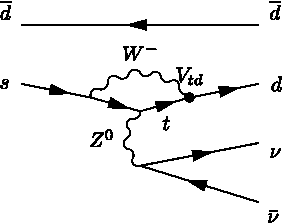
\includegraphics[height=3.5cm]{fig/penguin}
  \caption{A Feynman diagram.}
  \label{fig:Penguin}
\end{figure}

% starts a list of points to solve (a), (b), ...
\begin{exenumerate}
\item Stare at this equation for at least half an hour.
  \begin{align}
    A = B.
  \end{align}

\item Solve it.
  \hint{You might need to specify the unknown.}

  \begin{loesung}% the solution to this exercise part. \begin{solution} is the same
    The solution is given by ...... 
    \begin{align}
      A=B\ ,
    \end{align}
    of course.

    [Note that the equation in the solution has a separate numbering !]
  \end{loesung}
\end{exenumerate}


\begin{wrapfigure}{r}{45mm}
\centering
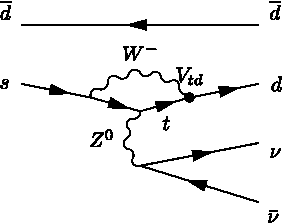
\includegraphics[width=40mm]{fig/penguin}
% You can have a caption here:
%\caption{A figure}
%\label{fig:Penguin2}
% Or, if you don't add a caption, wrapfig adds too much space, so you may remove it with a
% \vspace*{-length} command, like this: (You may have to play around with the spacing)
\vspace*{-10mm}
\end{wrapfigure}
Now you are required to study carefully the figure placed on the right side of this
paragraph, which was included using \texttt{wrapfig} and the
\verb|\begin{wrapfigure}...\end{wrapfigure}| environment.

\begin{exenumerate} % {exenumerate} environment automatically resumes correct numbering
\item Explain this diagram using words, describing which type of particle or antiparticle
  is incoming or outgoing, and specify all the symmetries.
\item Add all the missing momenta variables to this figure.
\end{exenumerate}
% small hack: break here the {exenumerate} environment, so that the follwing points that
% are below the wrapped figure go back to using the full page width.
\begin{exenumerate}
\item This diagram is very important, as it looks somewhat like a penguin. (Hence its
  name.) Calculate its cross-section to NNNNNNNLO.
\end{exenumerate}


% -------------------------------------------------------------------------
\uebung{Just a second exercise.}
\keywords{blah, blah, blah}

More stuff...

\begin{solution} % \begin{solution} and \begin{loesung} are the same
  The solution is summarized by the following diagram:
  \begin{center}
    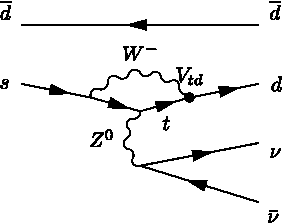
\includegraphics[angle=90,width=30mm]{fig/penguin}
  \end{center}
  One can easily see in the figure that the exercise was really easy.

  Other ways of solving the hard stuff are presented in Figs.~\ref{fig:SolPenguin}
  and~\ref{fig:SolPenguin2}.
  \begin{figure}
    \centering
    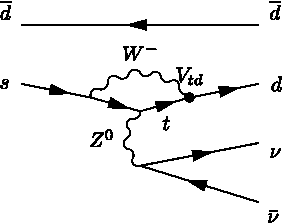
\includegraphics[angle=35,width=50mm]{fig/penguin}
    \caption{Solution Diagram.}
    \label{fig:SolPenguin}
  \end{figure}
  \begin{figure}[b] % you can use placement specifications, too
    \centering
    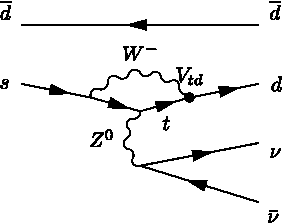
\includegraphics[angle=235,width=50mm]{fig/penguin}
    \caption{Solution Diagram.}
    \label{fig:SolPenguin2}
  \end{figure}
\end{solution}





\end{document}
